\documentclass[12pt,a4paper]{article}
\usepackage[utf8]{inputenc}
\usepackage[T1]{fontenc}
\usepackage[vietnamese]{babel}
\usepackage{geometry}
\geometry{
    a4paper,
    left=30mm,
    right=20mm,
    top=20mm,
    bottom=20mm
}
\usepackage{graphicx}
\usepackage{array}
\usepackage{amsmath}
\usepackage{booktabs}
\usepackage{color}
\usepackage[table,xcdraw]{xcolor}
\usepackage{caption}
\usepackage{enumitem}
\usepackage{indentfirst}
\usepackage{tabularx}
\usepackage{hyperref}

% Define colors matching the professional theme
\definecolor{navy}{HTML}{1B365D}
\definecolor{lightblue}{HTML}{336699}
\definecolor{tableheader}{HTML}{1B365D}
\definecolor{lightgray}{HTML}{F2F2F2}

\captionsetup{font=it, labelsep=colon}
\setlist[itemize]{noitemsep, topsep=3pt, parsep=3pt, partopsep=0pt}

\begin{document}

% --- Administrative Header ---
\begin{center}
    \textbf{\large CỘNG HÒA XÃ HỘI CHỦ NGHĨA VIỆT NAM}\\
    \textbf{\large Độc Lập - Tự Do - Hạnh Phúc}\\
    \small ---------------o0o---------------\\
    \vspace{2em}
    \textbf{\Large BẢN MÔ TẢ GIẢI PHÁP HỮU ÍCH}\\
    \vspace{1em}
    \textbf{\large Tên giải pháp: HỆ THỐNG HỖ TRỢ THỞ ÁP LỰC DƯƠNG TƯƠNG TÁC THÔNG MINH (SIPAP) TÍCH HỢP GIÁM SÁT ÁP SUẤT VÀ LƯỢNG KHÍ THỞ THỜI GIAN THỰC}
\end{center}

\vspace{1.5em}

\noindent Tên gọi sáng chế của thiết bị là \textbf{SIPAP (Smart Interactive PAP - Thiết bị hỗ trợ thở áp lực dương tương tác thông minh)}, là thuật ngữ thương hiệu và giải pháp cấu trúc do GS.TS.KH. Dương Quý Sỹ độc quyền sáng tạo và đề xuất bảo hộ quyền sở hữu trí tuệ, nhằm vinh danh sự đồng hành chuyên môn từ Hội Y học Giấc ngủ Việt Nam.

% --- Section I ---
\section{\textcolor{navy}{I. THÔNG TIN CHUNG VÀ CỐ VẤN KHOA HỌC}}
\begin{itemize}
    \item \textbf{Cố vấn khoa học \& Chỉ đạo chuyên môn:} GS. TS. KH. Dương Quý Sỹ (\textit{Chủ tịch Hội Y học Giấc ngủ Việt Nam - VSSM}).
    \item \textbf{Đơn vị bảo trợ học thuật và đồng hành chuyên môn:} Hội Y học Giấc ngủ Việt Nam (VSSM).
    \item \textbf{Nhóm tác giả nghiên cứu chế tạo:} GS.TS.KH. Dương Quý Sỹ, ThS. Trần Hữu Nam, ThS. Nguyễn Tuấn Anh, ThS. Tăng Thị Thảo Trâm, CN. Trần Thị Cẩm Tú, DS. Nguyễn Trọng Bằng, ThS. Nguyễn Văn Tới, TS. Nguyễn Duy Thái, GS. Ramon Farré, GS.TS. Thomas Penzel, GS.TS. Francis Martin, GS. Đinh Xuân Anh Tuấn.
\end{itemize}

\begin{figure}[h!]
    \centering
    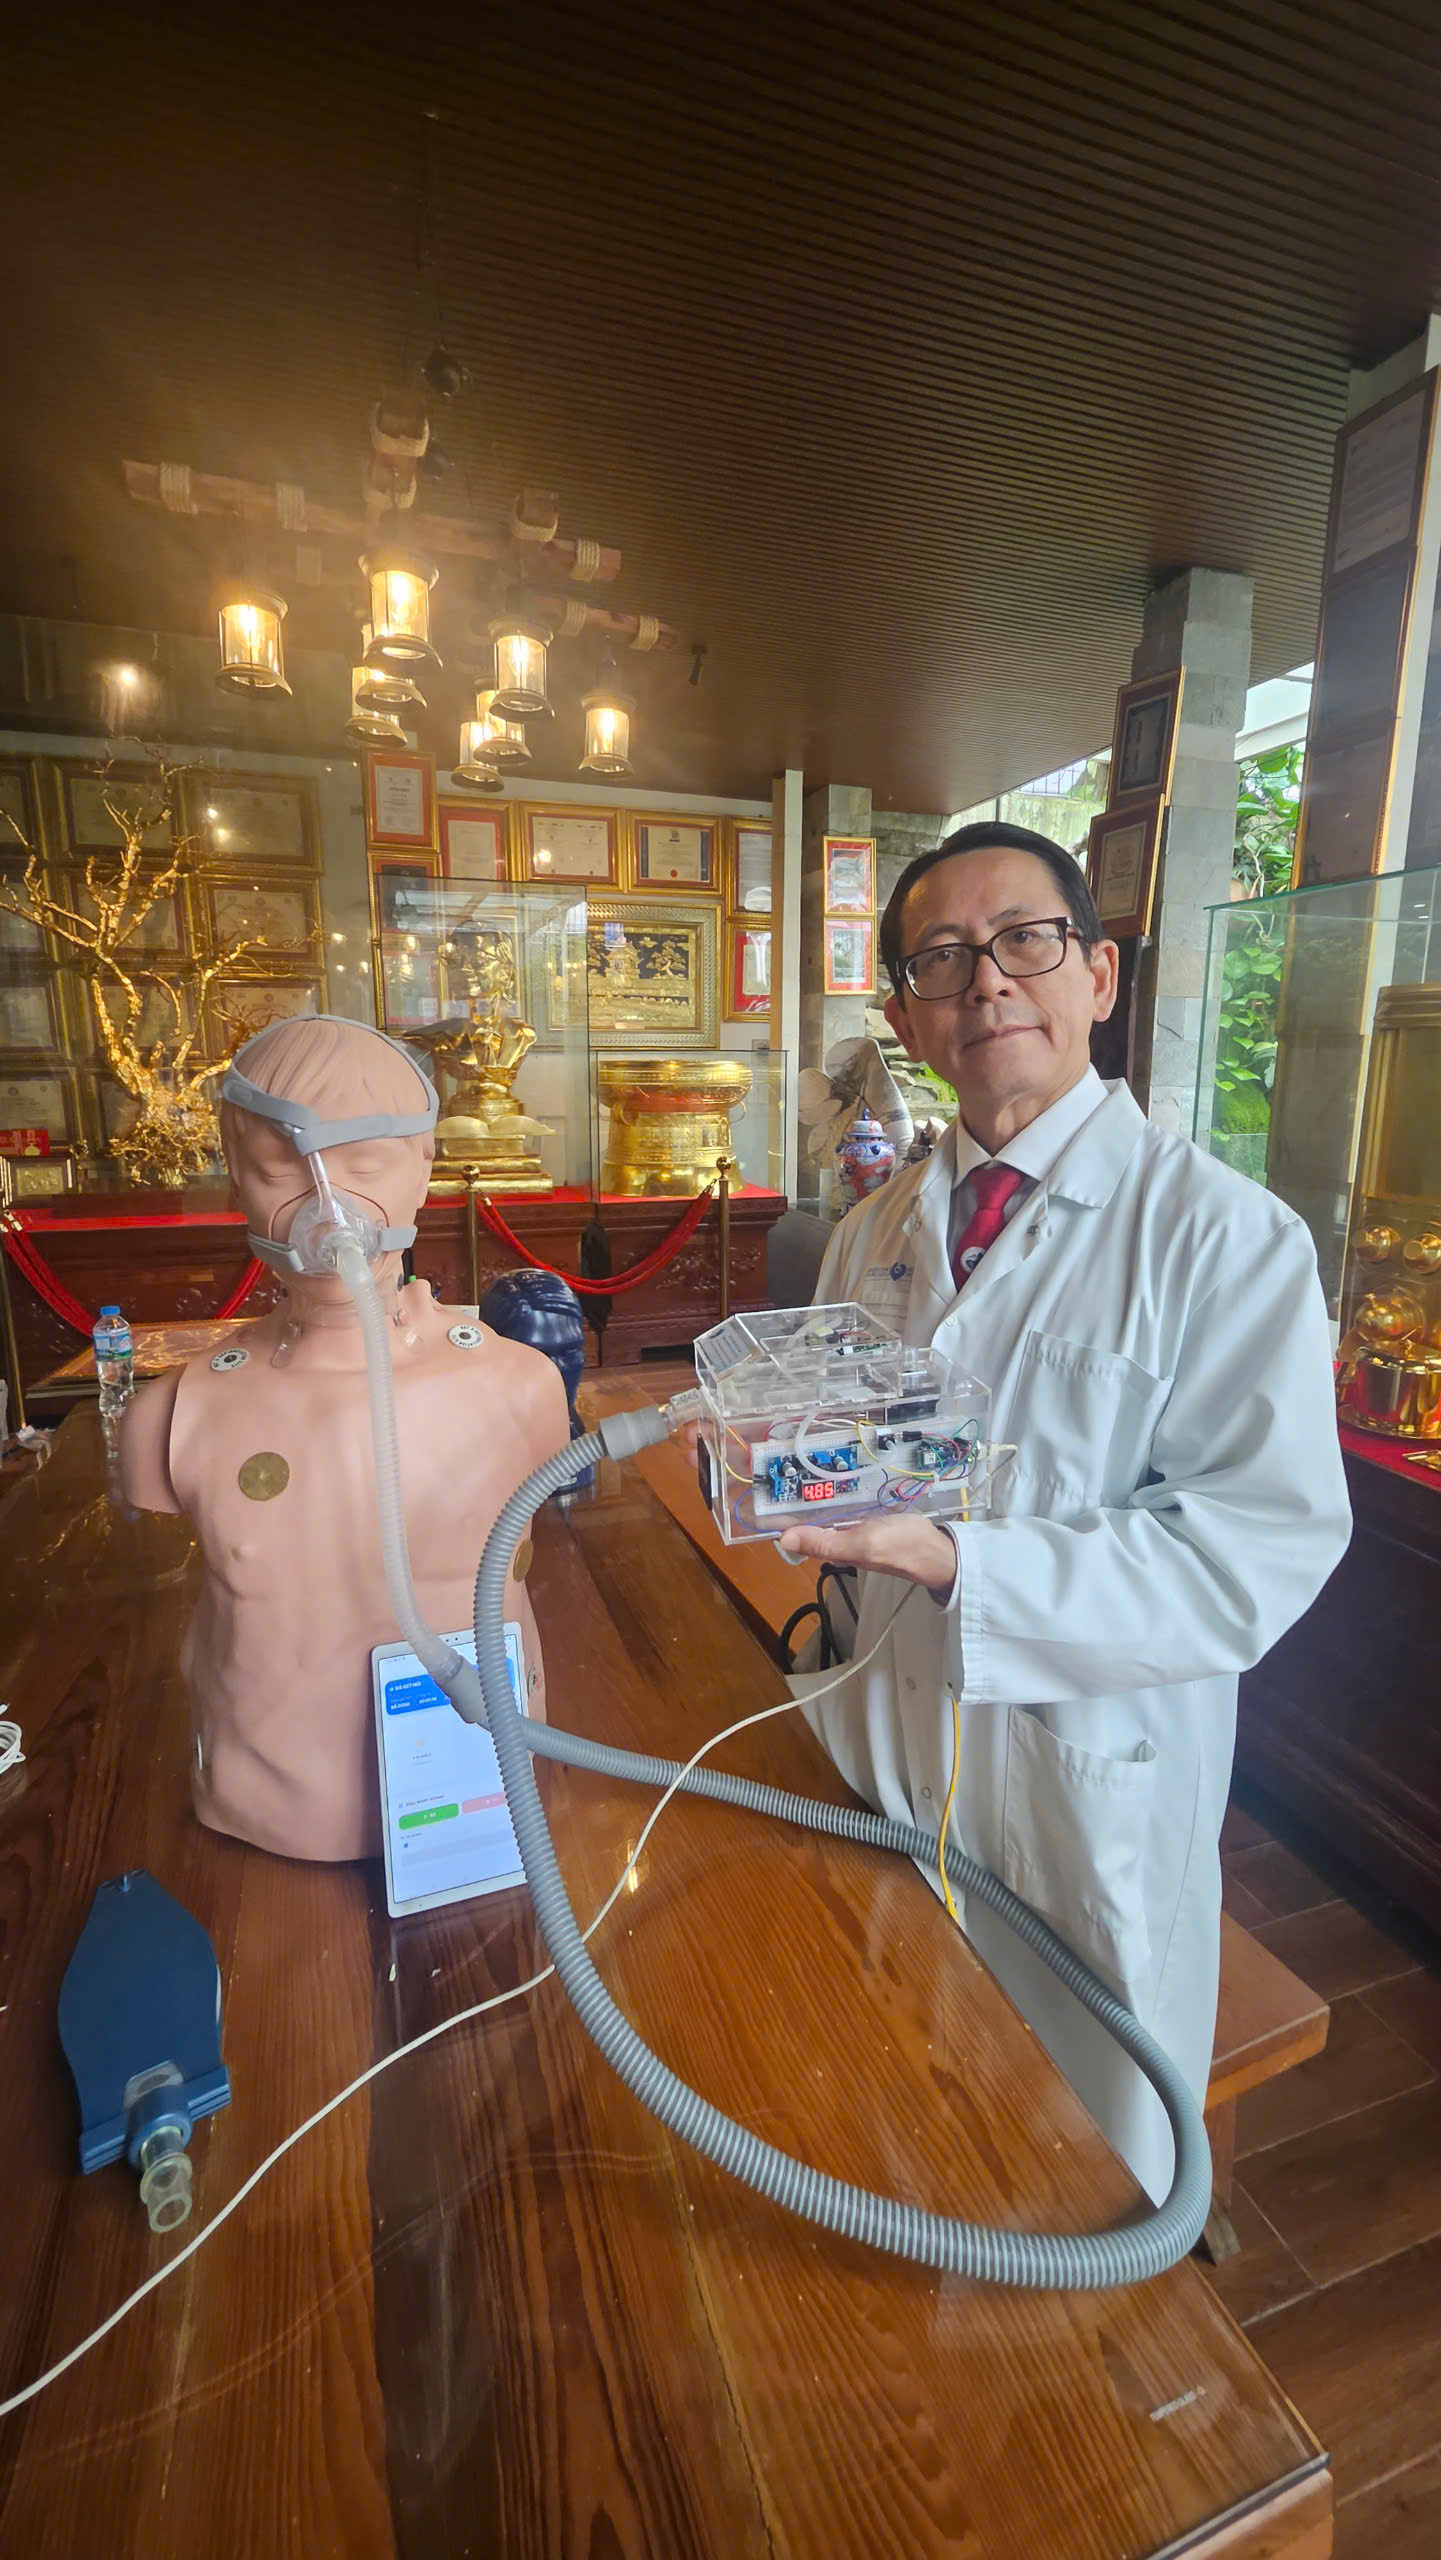
\includegraphics[width=0.7\textwidth]{image_3.png}
    \caption{GS. TS. KH. Dương Quý Sỹ kiểm tra mẫu thiết kế thực tế của thiết bị hỗ trợ thở tương tác thông minh SIPAP.}
    \label{fig:fig1}
\end{figure}

% --- Section II ---
\section{\textcolor{navy}{II. LĨNH VỰC KỸ THUẬT ĐƯỢC ĐỀ CẬP}}
Giải pháp hữu ích này đề cập đến lĩnh vực thiết bị y tế hỗ trợ chức năng hô hấp, cụ thể là hệ thống hỗ trợ thở áp lực dương liên tục (Continuous Positive Airway Pressure - CPAP) có khả năng tương tác thông minh (Smart \& Interactive PAP - viết tắt là SIPAP). Hệ thống này phục vụ mục đích hỗ trợ thở không xâm lấn nhằm điều trị và quản lý tại nhà hoặc bệnh viện cho các bệnh nhân mắc hội chứng ngưng thở khi ngủ do tắc nghẽn (Obstructive Sleep Apnea - OSA).

% --- Section III ---
\section{\textcolor{navy}{III. TÌNH TRẠNG KỸ THUẬT CỦA GIẢI PHÁP HỮU ÍCH}}
Theo các thống kê y tế gần đây, tại Việt Nam có khoảng 4 triệu người trưởng thành mắc hội chứng ngưng thở khi ngủ do tắc nghẽn (OSA), chiếm tỷ lệ khoảng 8.5\% dân số. Trong đó, có khoảng 2.3 triệu bệnh nhân ở mức độ trung bình đến nặng - là nhóm đối tượng có nguy cơ cao gặp các biến chứng nguy hiểm về tim mạch (tăng huyết áp, đột quỵ, nhồi máu cơ tim) và tai nạn lao động do buồn ngủ ban ngày. Phương pháp điều trị chuẩn và hiệu quả nhất là sử dụng máy thở áp lực dương liên tục (CPAP) trong lúc ngủ để duy trì đường thở luôn thông thoáng.

Tuy nhiên, các máy CPAP thương mại hiện hành tại Việt Nam đối mặt với các nhược điểm lớn sau:
\begin{itemize}
    \item Chi phí nhập khẩu rất cao (dao động từ 15 đến hơn 50 triệu đồng), vượt quá khả năng chi trả của phần lớn người dân lao động.
    \item Hệ thống đóng kín, không thể cá nhân hóa phần cứng hoặc nâng cấp các module cảm biến bổ sung tùy biến theo nhu cầu lâm sàng.
    \item Thiếu khả năng kết nối trực tiếp thời gian thực với các thiết bị di động cá nhân và đồng bộ dữ liệu y tế với hệ thống theo dõi sức khỏe từ xa (SleepCare), gây khó khăn cho các bác sĩ trong việc giám sát sự tuân thủ điều trị của bệnh nhân tại nhà.
    \item Một số dòng máy giá rẻ không tích hợp sẵn cảm biến lưu lượng khí thở độ nhạy cao (Flow Sensor) hoặc cảm biến bão hòa oxy máu ($SpO_2$) trực tiếp trên cùng một hệ thống để tính toán đồng bộ chỉ số giảm thở AHI (Apnea-Hypopnea Index) của bệnh nhân.
\end{itemize}

% --- Section IV ---
\section{\textcolor{navy}{IV. BẢN CHẤT KỸ THUẬT CỦA GIẢI PHÁP HỮU ÍCH}}
Để giải quyết các hạn chế nêu trên, giải pháp hữu ích đề xuất một hệ thống CPAP thông minh (SIPAP) có cấu trúc module hóa cao, tích hợp đồng bộ đa cảm biến và giao tiếp không dây năng lượng thấp (Bluetooth Low Energy - BLE). Hệ thống được thiết kế hướng tới tối ưu hóa chi phí sản xuất, sử dụng các linh kiện phù hợp nhưng vẫn đảm bảo độ chính xác y tế.

\subsection{Các tính năng và chế độ hoạt động chính:}
\begin{itemize}
    \item Hệ thống hỗ trợ 3 chế độ thở cơ bản tùy biến qua phần mềm: CPAP/AutoCPAP (áp lực dương cố định hoặc tự động điều chỉnh áp lực), BiPAP (cung cấp hai mức áp lực riêng biệt IPAP khi hít vào và EPAP khi thở ra để giảm công hô hấp) và APAP (phân tích tắc nghẽn đường thở thời gian thực để thay đổi áp suất tối ưu).
    \item Dải áp lực điều trị ổn định: từ 4 đến 25 $cmH_2O$, được điều tiết liên tục dựa trên thuật toán điều khiển vòng kín tốc độ quạt (RPM).
    \item Tích hợp cảm biến áp suất MPXV5010G đo áp suất đường thở thực tế tại vị trí mặt nạ với độ nhạy cao.
    \item Tích hợp cảm biến lưu lượng SFM3300-D đo lưu lượng dòng khí thở tức thời của bệnh nhân để xác định nhịp thở, phát hiện cơn ngừng thở hoặc giảm thở.
    \item Thiết kế dự phòng sẵn cổng kết nối cho cảm biến đo nồng độ bão hòa oxy máu ($SpO_2$) nhằm phục vụ việc nâng cấp tích hợp ở phiên bản tiếp theo.
    \item Giao diện người dùng tại chỗ trực quan thông qua màn hình OLED hiển thị thông số và nút xoay mã hóa vòng quay (Rotary Encoder) kết hợp nút nhấn.
    \item Kết nối không dây BLE GATT Profile với tên thiết bị "SIPAP" truyền gói dữ liệu JSON mỗi 200ms lên ứng dụng di động để đồng bộ với đám mây SleepCare.
    \item Tích hợp bình làm ẩm (Humidifier module) chứa nước cất trên đường thở giúp duy trì độ ẩm và nhiệt độ thích hợp cho luồng khí cung cấp tới bệnh nhân, giảm kích ứng và khô rát niêm mạc hô hấp của người sử dụng.
\end{itemize}

\begin{figure}[h!]
    \centering
    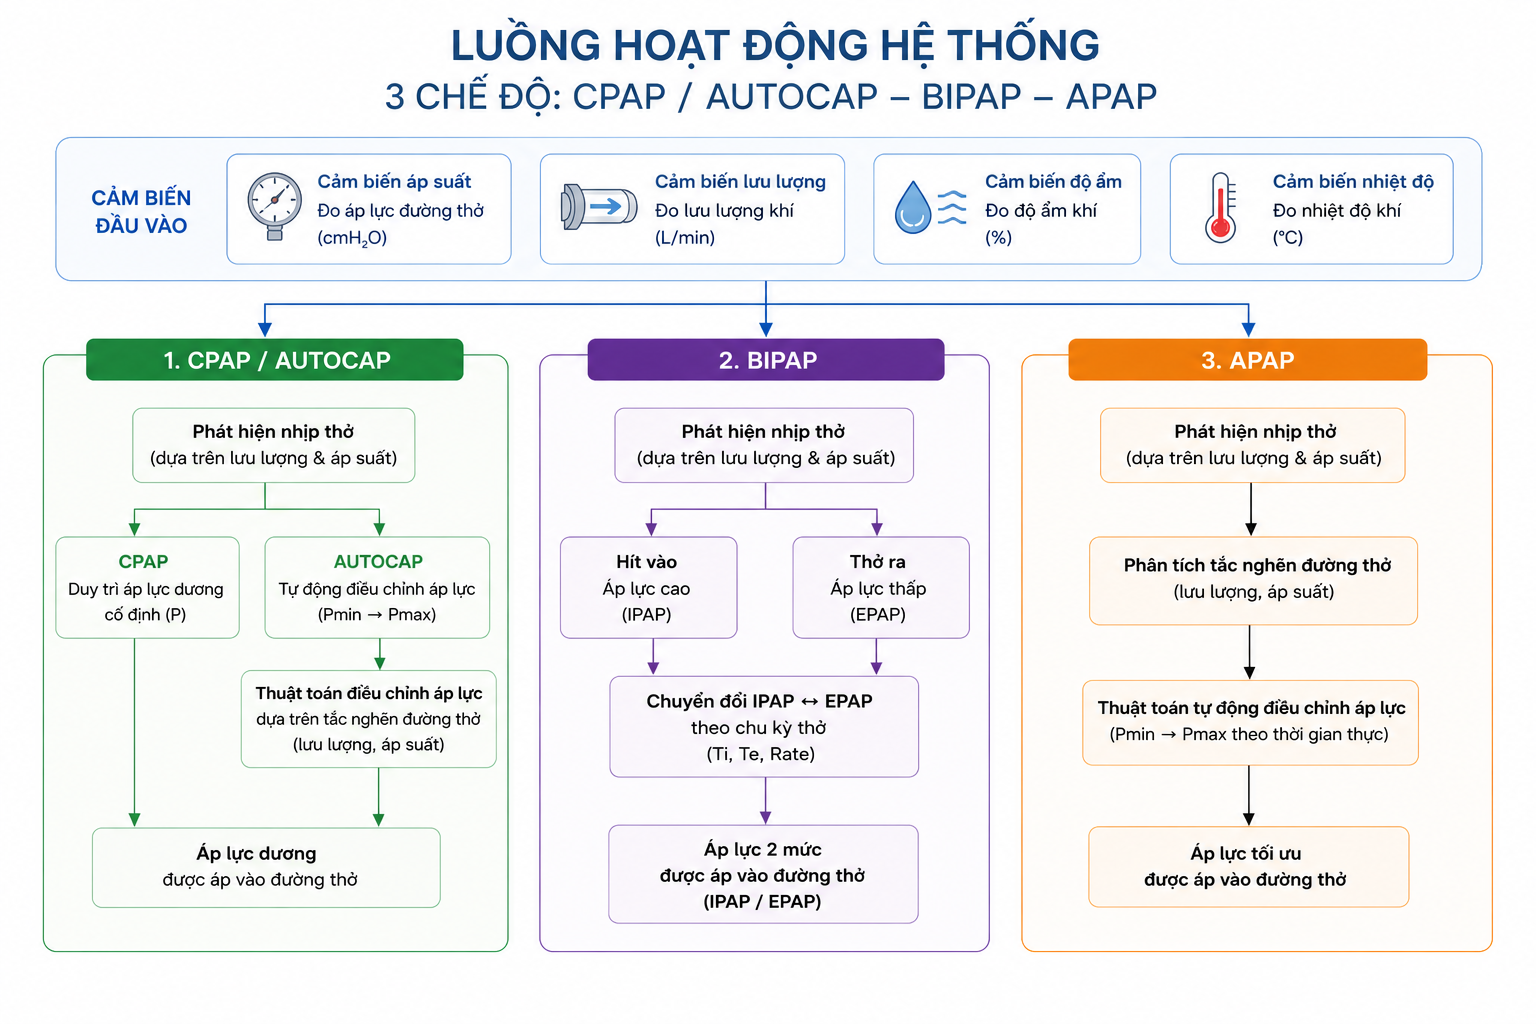
\includegraphics[width=0.8\textwidth]{image.png}
    \caption{Sơ đồ luồng hoạt động của hệ thống hỗ trợ thở SIPAP với 3 chế độ CPAP, BiPAP và APAP.}
    \label{fig:fig2}
\end{figure}

% --- Section V ---
\section{\textcolor{navy}{V. MÔ TẢ CHI TIẾT PHƯƠNG ÁN THỰC HIỆN}}

\subsection{Sơ đồ cấu trúc phần cứng hệ thống}
Hệ thống bao gồm các khối chức năng chính được kết nối và phối hợp vận hành như sau:
\begin{itemize}
    \item \textbf{Khối cảm biến thu thập dữ liệu sinh hiệu:} Cảm biến áp suất MPXV5010G và cảm biến lưu lượng SFM3300-D là hai cảm biến hoạt động chính trong phiên bản 1 để đo áp suất mặt nạ và lưu lượng khí thở thực tế. Các cảm biến phụ trợ khác như cảm biến nhiệt độ \& độ ẩm không khí SHT30/SHT31, cảm biến $SpO_2$ được thiết kế sẵn cổng kết nối chờ để phục vụ nâng cấp ở các phiên bản tiếp theo.
    \item \textbf{Khối xử lý trung tâm:} Vi điều khiển chính Arduino Nano 33 BLE Sense (sử dụng chip ARM Cortex-M4 32-bit mạnh mẽ, tích hợp sẵn anten BLE) thực hiện việc đọc dữ liệu cảm biến, chạy thuật toán điều khiển PID quạt và phát sóng BLE. Vi điều khiển phụ ESP32 được dự phòng tích hợp trên bo mạch để thực hiện kết nối Wi-Fi/Internet gửi dữ liệu trực tiếp lên Cloud IoT.
    \item \textbf{Khối tạo áp lực:} Sử dụng động cơ quạt thổi không chổi than (Brushless Blower) WS4540-12-NZ03 hoạt động ở điện áp 12VDC, kèm Driver điều khiển chuyên dụng. Driver nhận xung PWM từ chân D3 của Arduino để thay đổi tốc độ quay, đồng thời gửi lại xung phản hồi tốc độ quay FG về chân ngắt D2 của Arduino.
    \item \textbf{Khối đường dẫn khí:} Bao gồm buồng khí chế tạo từ vật liệu Mica trong dày 3mm cắt laser chính xác, ống dẫn khí silicon y tế mềm, mặt nạ thở dạng mũi (nasal mask) và van thở ra (exhalation valve).
    \item \textbf{Khối làm ẩm (Humidifier):} Tích hợp bình làm ẩm chứa nước y tế nằm tiếp nối ngay sau quạt thổi khí và trước mặt nạ thở. Khí áp lực dương đi qua bề mặt nước để hấp thụ hơi ẩm khuếch tán tự nhiên trước khi đi vào đường hô hấp của bệnh nhân.
    \item \textbf{Khối nguồn:} Adapter 12VDC công suất lớn cấp cho động cơ blower; mạch hạ áp Buck Converter bước xuống 5V và 3.3V có độ ổn định cao để nuôi vi điều khiển và các cảm biến tránh nhiễu tín hiệu analog.
    \item \textbf{Khối giao diện:} Màn hình OLED kết hợp bộ mã hóa quay (Rotary Encoder) 8 nút xoay và nút ấn để người dùng cài đặt thông số áp suất đích và chế độ thở tại chỗ.
\end{itemize}

\begin{figure}[h!]
    \centering
    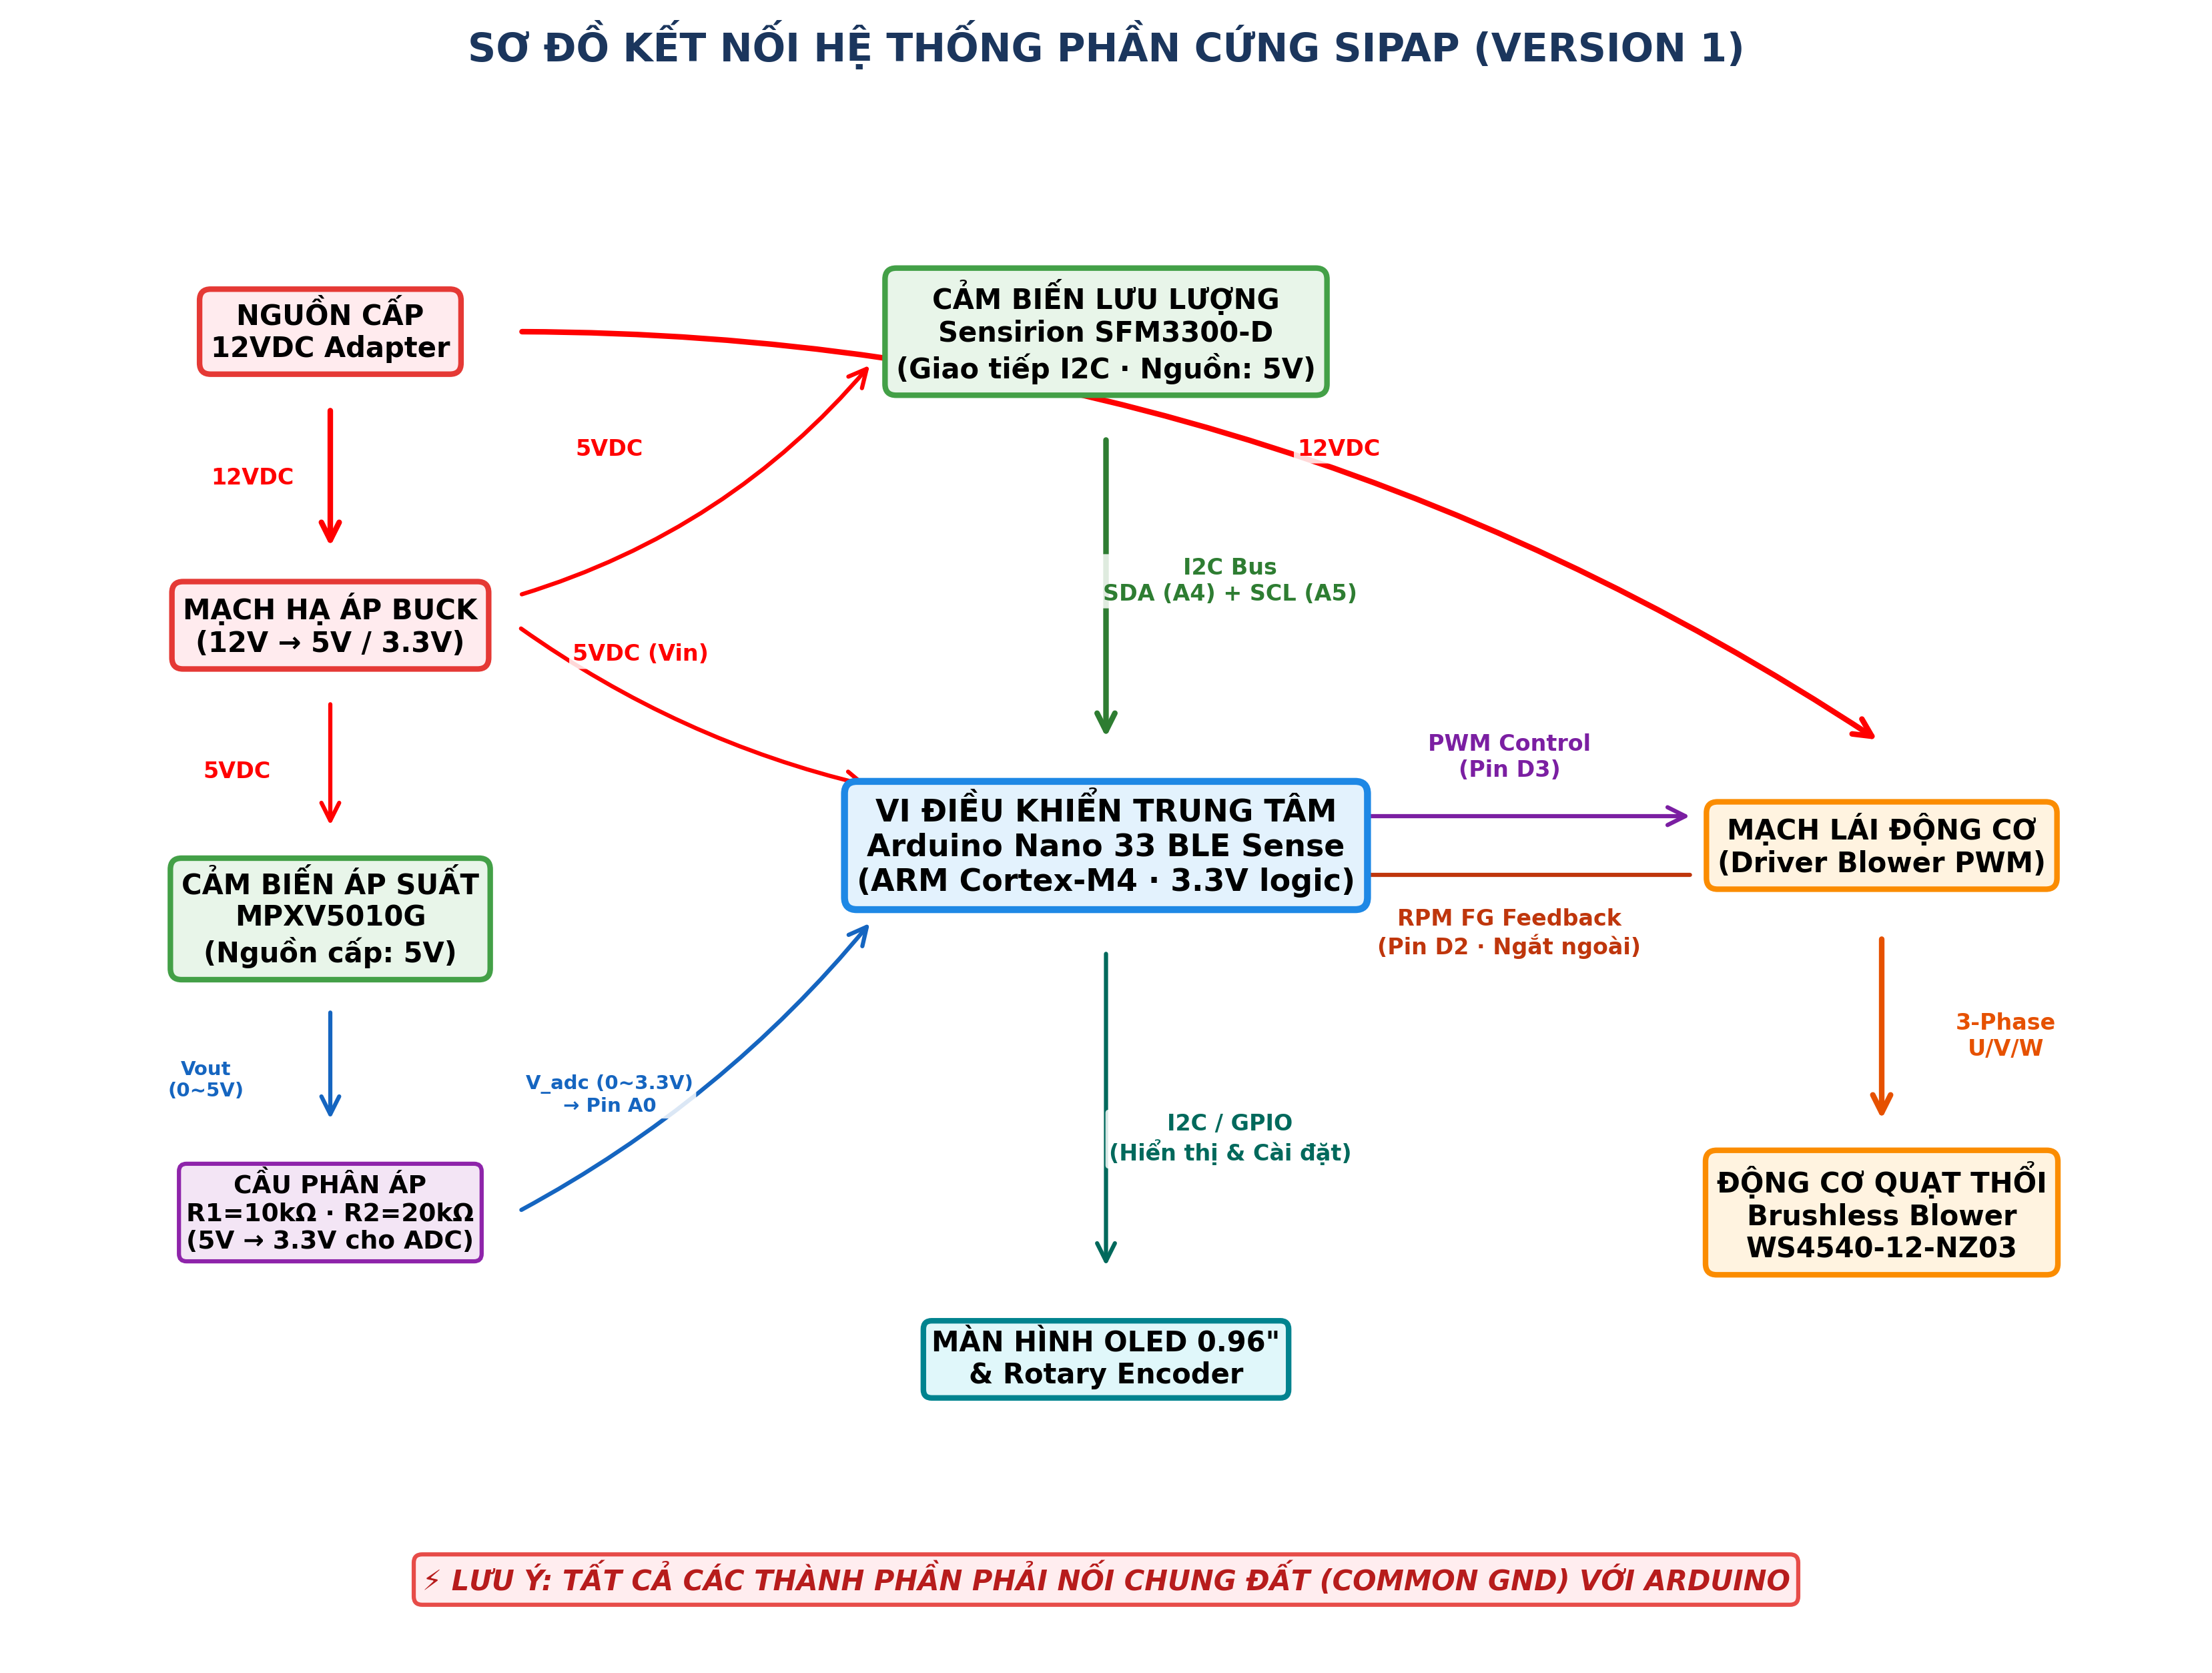
\includegraphics[width=0.8\textwidth]{schematic.png}
    \caption{Sơ đồ kết nối phần cứng và phân bổ chân tín hiệu giữa các thành phần của hệ thống SIPAP.}
    \label{fig:fig3}
\end{figure}

\begin{figure}[h!]
    \centering
    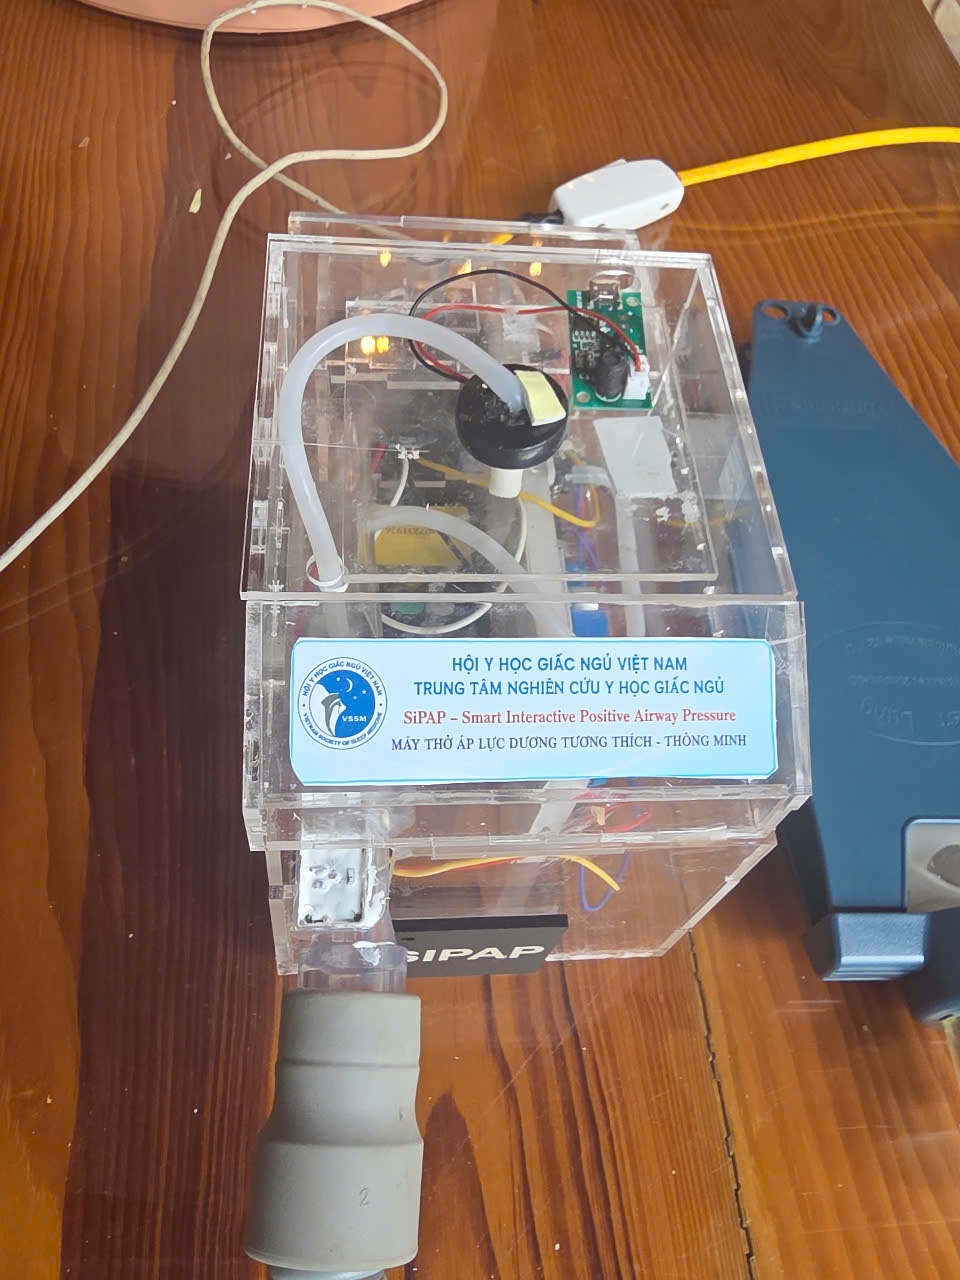
\includegraphics[width=0.7\textwidth]{image_4.png}
    \caption{Thiết bị thực tế SIPAP cận cảnh cấu trúc buồng khí và cách bố trí các module bo mạch.}
    \label{fig:fig4}
\end{figure}

\begin{figure}[h!]
    \centering
    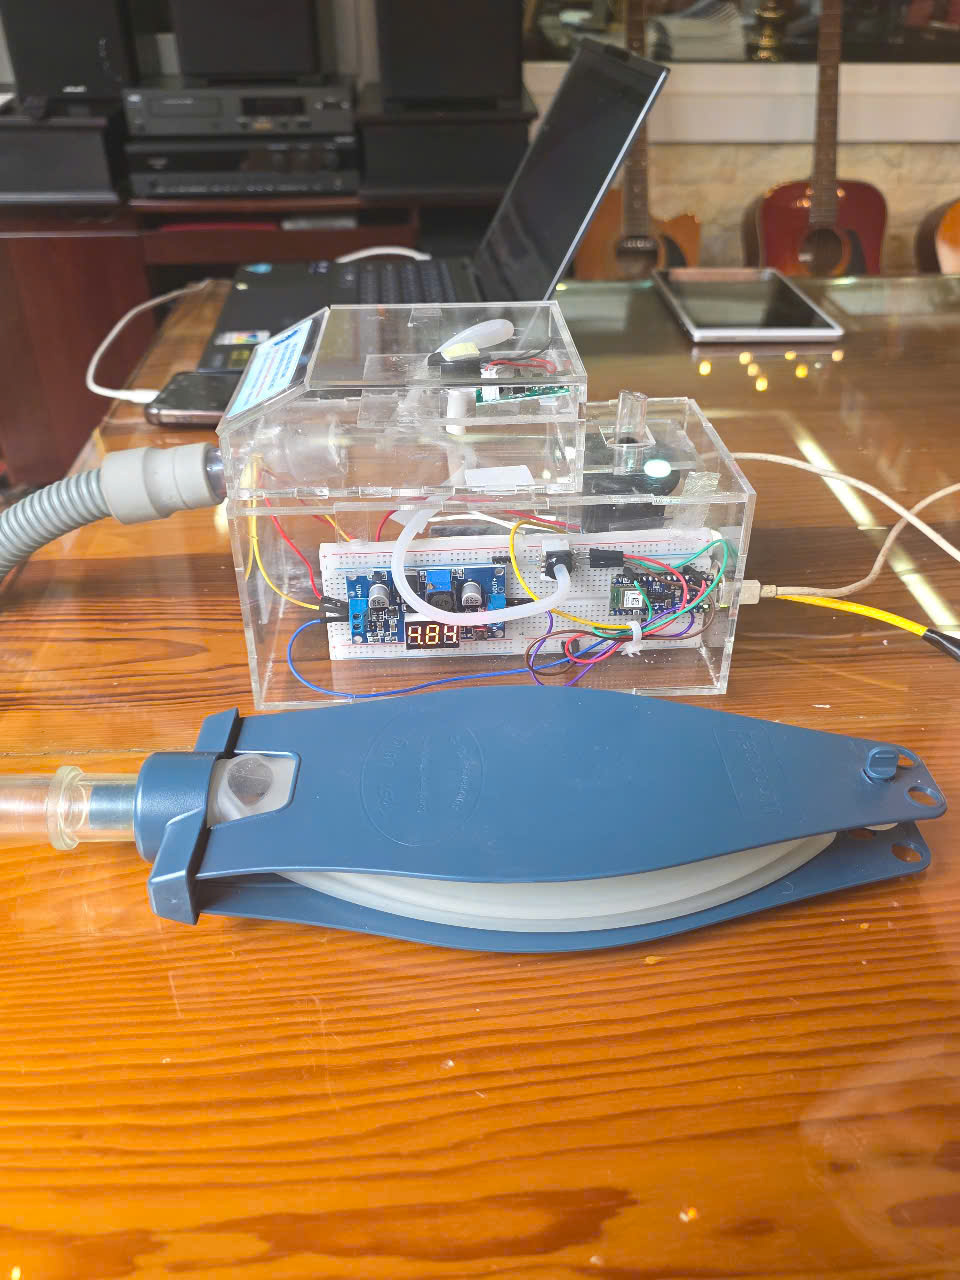
\includegraphics[width=0.7\textwidth]{image_1.png}
    \caption{Mẫu thử nghiệm hoàn chỉnh của thiết bị SIPAP kết nối với bóng thở (phổi giả) phục vụ kiểm định hiệu năng quạt thổi.}
    \label{fig:fig5}
\end{figure}

\newpage
\subsection{Chi tiết thông số kỹ thuật của các cấu phần cốt lõi}

\subsubsection*{a) Động cơ quạt thổi không chổi than (Brushless Blower WS4540-12-NZ03)}
Đây là bộ phận cốt lõi của khối tạo áp lực, tạo ra lưu lượng và áp suất dương cần thiết cho đường dẫn khí. Các thông số đặc tính vận hành bao gồm:
\begin{itemize}
    \item Mã thiết bị (Part No): WS4540-12-NZ03.
    \item Điện áp định mức (Voltage): 12 VDC.
    \item Vận hành tại điểm Lưu lượng khí cực đại (At Max Air flow): Tốc độ quay đạt 45.000 vòng/phút (RPM); Dòng điện tiêu thụ 1,6 A; Công suất tiêu thụ 119,2 W; Lưu lượng khí đạt 7,2 $m^3$/h (tương đương 4,23 CFM hoặc 120 LPM); Độ ồn đo được là 62 dBA.
    \item Vận hành tại điểm Á suất khí cực đại (At Max Air Pressure): Tốc độ quay đạt 49.000 vòng/phút (RPM); Dòng điện tiêu thụ 0,9 A; Công suất tiêu thụ 10,8 W; Áp suất tĩnh đạt 5,0 kPa (tương đương 51 $cmH_2O$); Độ ồn khi bị chặn hoàn toàn dòng khí (Block Noise Level) là 49 dBA.
\end{itemize}

\begin{figure}[h!]
    \centering
    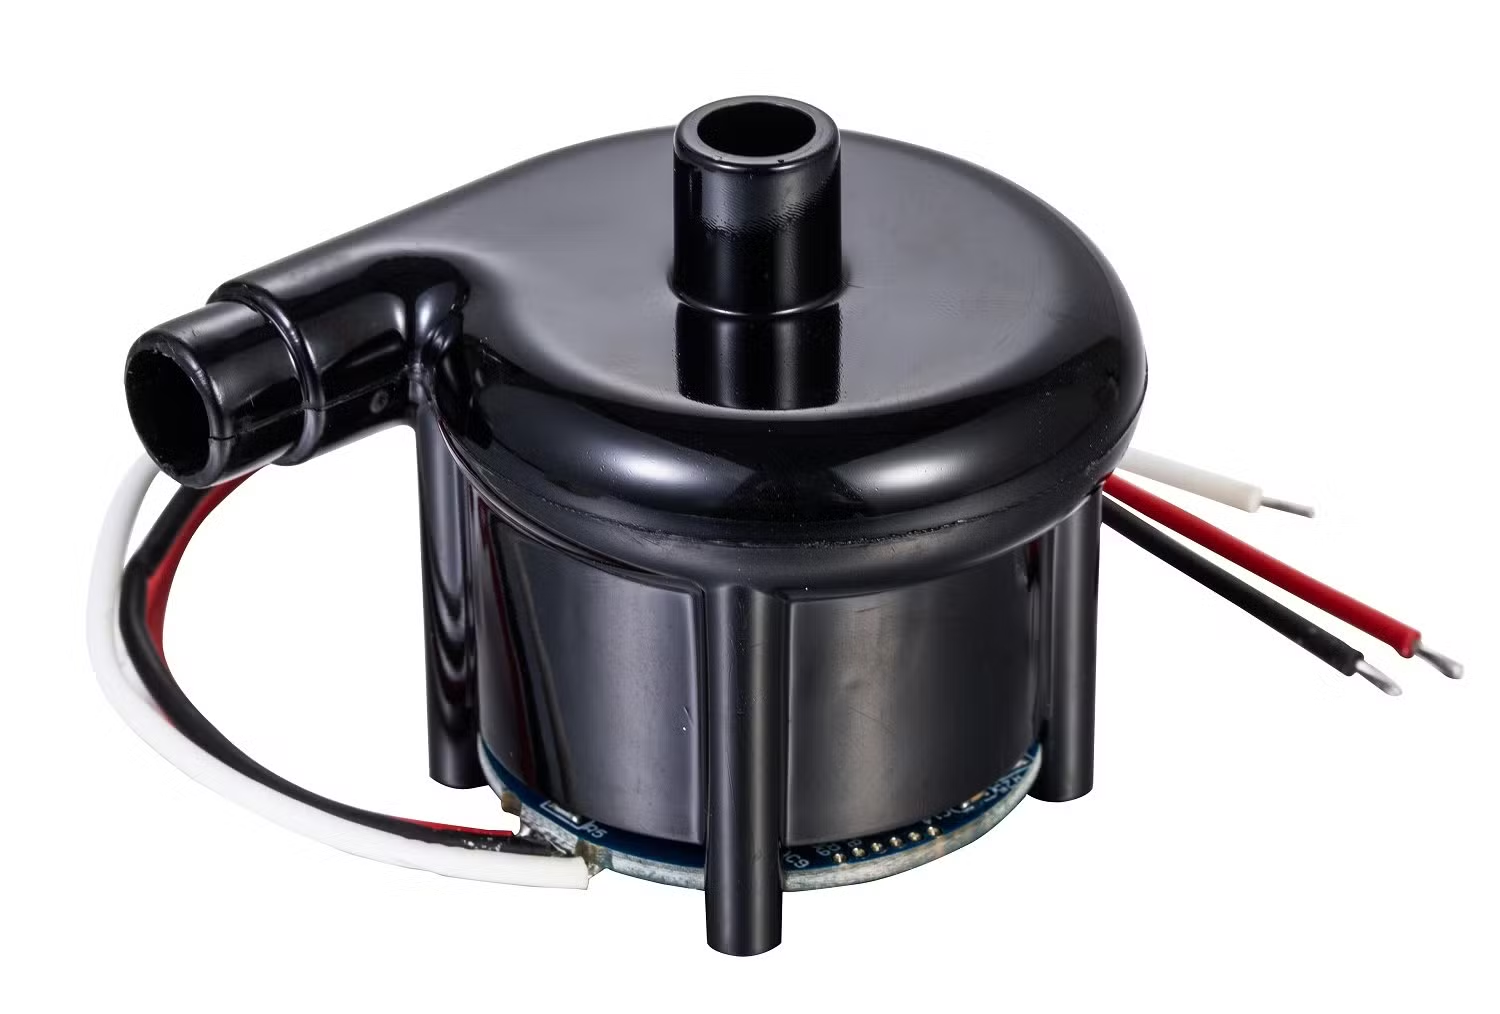
\includegraphics[width=0.5\textwidth]{blower.png}
    \caption{Động cơ quạt thổi không chổi than WS4540-12-NZ03 sử dụng trong khối tạo áp lực.}
    \label{fig:fig6}
\end{figure}

\subsubsection*{b) Cảm biến áp suất đường thở (MPXV5010G)}
Cảm biến silicon piezoresistive chuyên dụng để đo áp suất đường thở tại mặt nạ thở. Thông số đặc tính kỹ thuật bao gồm:
\begin{itemize}
    \item Dải đo áp suất (POP): 0 đến 10 kPa (tương đương 0 đến 1019,78 $mmH_2O$ hoặc 0 đến 100 $cmH_2O$).
    \item Điện áp cấp ($V_S$): 4,75 VDC đến 5,25 VDC (Mức định mức 5,0 VDC).
    \item Dòng điện tiêu thụ ($I_o$): tối đa 10 mAdc (điển hình 5,0 mAdc).
    \item Điện áp điểm không ($V_{\text{off}}$): 0,2 VDC (điển hình) tại áp suất 0 kPa.
    \item Điện áp đầu ra cực đại ($V_{\text{FSO}}$): 4,7 VDC (điển hình) tại áp suất 10 kPa.
    \item Hiệu số điện áp toàn dải ($V_{\text{FSS}}$): 4,5 VDC (điển hình).
    \item Độ chính xác (Accuracy): sai số trong khoảng $\pm$5,0\% $V_{\text{FSS}}$ trong dải nhiệt độ vận hành từ 0 đến 85$^\circ$C.
    \item Độ nhạy (Sensitivity): 450 mV/kPa (hoặc 4,413 mV/$mmH_2O$).
    \item Thời gian đáp ứng (Response Time): 1,0 ms.
    \item Thời gian khởi động ổn định (Warm-Up Time): 20 ms.
    \item Áp suất chịu đựng tối đa trước khi hỏng ($P_{\text{max}}$): 40 kPa.
\end{itemize}

\begin{figure}[h!]
    \centering
    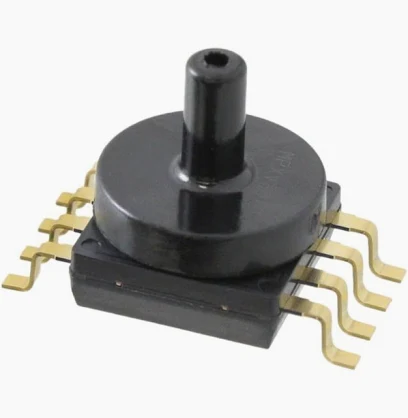
\includegraphics[width=0.5\textwidth]{sensorpressure.png}
    \caption{Cảm biến áp suất silicon MPXV5010G với kết cấu chân dán SOP.}
    \label{fig:fig7}
\end{figure}

\subsubsection*{c) Cảm biến lưu lượng khí thở (Sensirion SFM3300-D / SFM3300-AW)}
Lưu lượng kế kỹ thuật số chuyên dụng đo dòng khí hô hấp y tế. Thông số đặc tính kỹ thuật bao gồm:
\begin{itemize}
    \item Dải đo lưu lượng: -250 đến +250 slm (Đo hai chiều).
    \item Khoảng chết (Dead space): cực nhỏ, dưới 10 ml.
    \item Độ phân giải đầu ra: 14 bit.
    \item Chu kỳ cập nhật dữ liệu (Update Time): cực nhanh, chỉ 0,5 ms.
    \item Giao tiếp truyền thông: Giao thức I2C, Địa chỉ mặc định (Default Sensor Address): 64 (0x40 ở hệ cơ số 16).
    \item Điện áp hoạt động: 5 VDC $\pm$5\%.
    \item Công suất tiêu thụ: dưới 50 mW.
    \item Hệ số tỉ lệ dòng (Scale Factor Flow): 120 $\text{slm}^{-1}$.
    \item Giá trị điểm không (Offset Flow): 32768.
    \item Dải áp suất tuyệt đối hoạt động: 0,54 đến 1,1 bar.
\end{itemize}

\begin{figure}[h!]
    \centering
    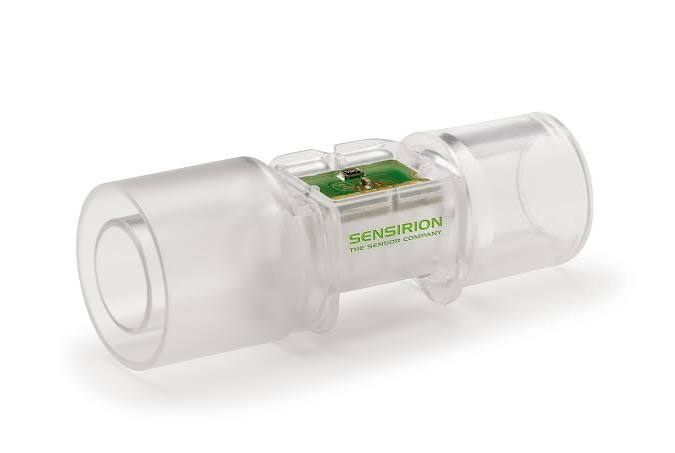
\includegraphics[width=0.5\textwidth]{sensorflow.png}
    \caption{Cảm biến lưu lượng khí y tế chuyên dụng Sensirion SFM3300-D.}
    \label{fig:fig8}
\end{figure}

\subsection{Danh mục vật tư chế tạo mẫu thử nghiệm (BOM)}
Dưới đây là bảng liệt kê danh mục vật tư chế tạo hệ thống máy thở tương tác thông minh SIPAP được lập cho phiên bản thử nghiệm - dự kiến:

\vspace{1em}
\noindent
\begin{tabularx}{\textwidth}{|>{\centering\arraybackslash}p{0.8cm}|>{\raggedright\arraybackslash}p{4.0cm}|>{\centering\arraybackslash}p{0.8cm}|>{\raggedleft\arraybackslash}p{2.2cm}|>{\raggedleft\arraybackslash}p{2.2cm}|>{\raggedright\arraybackslash}X|}
\hline
\rowcolor{navy}
\textbf{\textcolor{white}{STT}} & \textbf{\textcolor{white}{Tên Linh Kiện}} & \textbf{\textcolor{white}{SL}} & \textbf{\textcolor{white}{Đơn giá (VND)}} & \textbf{\textcolor{white}{Thành tiền (VND)}} & \textbf{\textcolor{white}{Ghi chú}} \\ \hline
1 & Arduino Nano 33 BLE Sense & 1 & 863.000 & 863.000 & Vi điều khiển chính, ARM Cortex-M4, tích hợp BLE \\ \hline
2 & ESP32 Microcontroller (chưa dùng) & 1 & 162.000 & 162.000 & Vi điều khiển phụ phục vụ mở rộng WiFi (dự phòng nâng cấp) \\ \hline
3 & Nguồn 12 V & 1 & 100.000 & 100.000 & Cấp nguồn 12VDC cho quạt thổi và Driver \\ \hline
4 & Rắc chuyển đổi & 1 & 50.000 & 50.000 & Đầu giắc cắm DC Power Jack 5.5x2.1mm \\ \hline
5 & Mạch hạ áp (Buck) & 1 & 50.000 & 50.000 & Hạ áp từ 12V sang 5V/3.3V cấp cho MCU \& cảm biến \\ \hline
6 & Cáp nối, dây điện, keo dán & 1 & 50.000 & 50.000 & Vật tư kết nối mạch và cố định linh kiện cơ khí \\ \hline
7 & Cảm biến áp suất (MPXV5010G) & 1 & 673.000 & 673.000 & Cảm biến áp suất silicon đo áp suất mask (0-10 kPa) \\ \hline
8 & Motor Blower \& Driver (WS4540-12-NZ03) & 1 & 1.142.000 & 1.142.000 & Động cơ thổi áp suất cao 12VDC và Driver PWM \\ \hline
9 & Mặt nạ mũi (Nasal Mask) & 1 & 1.000.000 & 1.000.000 & Mặt nạ thở silicon y tế đeo mũi của bệnh nhân \\ \hline
10 & Mica trong + công cắt laser & 1 & 500.000 & 500.000 & Chế tạo hộp vỏ máy và buồng nén khí \\ \hline
11 & Cảm biến đo nồng độ SpO2 (chưa dùng) & 1 & 100.000 & 100.000 & Cảm biến quang học đo nồng độ oxy huyết (dự phòng nâng cấp cho phiên bản sau) \\ \hline
12 & Màn hình hiển thị OLED & 1 & 65.000 & 65.000 & Màn hình hiển thị thông số áp suất, lưu lượng, nhịp thở \\ \hline
13 & Cảm biến lưu lượng (SFM3300-D) & 1 & 2.300.000 & 2.300.000 & Cảm biến lưu lượng khí y tế chuyên dụng, giao tiếp I2C \\ \hline
14 & Nút xoay và nút ấn (Rotary Encoder) & 1 & 40.000 & 40.000 & Bộ mã hóa vòng quay tương tác người dùng tại chỗ \\ \hline
15 & Bình làm ẩm khí thở (Humidifier) & 1 & 250.000 & 250.000 & Bình chứa nước y tế làm ẩm luồng khí thở tự nhiên \\ \hline
\rowcolor{lightgray}
\multicolumn{4}{|c|}{\textbf{TỔNG CỘNG CHI PHÍ VẬT TƯ CHẾ TẠO}} & \textbf{7.345.000} & \textit{\small Đã bao gồm VAT và công cắt vỏ mica} \\ \hline
\end{tabularx}

\vspace{1.5em}

\subsection{Giải thuật điều khiển và hoạt động của phần mềm}
Hoạt động xử lý thời gian thực của thiết bị được lập trình tối ưu hóa trên nền tảng vi điều khiển. Dựa trên mã nguồn firmware thực tế (\texttt{dull.ino}), nguyên lý xử lý số liệu được thực thi như sau:

\begin{itemize}
    \item \textbf{Kiểm chứng thuật toán tính toán áp suất từ cảm biến MPXV5010G:}
    Hàm đọc dữ liệu cảm biến áp suất trong mã nguồn \texttt{dull.ino} sử dụng công thức chuyển đổi từ giá trị ADC sang giá trị áp suất thực tế (kPa):
    \begin{equation}
        \text{pressure} = \frac{\frac{\text{sensorVoltage}}{5.0} - 0.04}{0.09}
    \end{equation}
    Phương trình này hoàn toàn chính xác về mặt toán học và vật lý học, được chứng minh dựa trên thông số từ datasheet của nhà sản xuất:
    \begin{itemize}
        \item Theo tài liệu kỹ thuật MPXV5010G, hàm truyền đặc tính ngõ ra lý thuyết (với nguồn nuôi $V_s = 5.0$ Vdc, nhiệt độ $T_A = 25^\circ$C) là:
        \begin{equation}
            V_{\text{out}} = V_s \times (0.09 \times P + 0.04)
        \end{equation}
        trong đó $P$ là áp suất đầu vào đo bằng kPa.
        \item Thực hiện biến đổi toán học tìm $P$ từ điện áp ngõ ra $V_{\text{out}}$:
        \begin{align}
            \frac{V_{\text{out}}}{V_s} &= 0.09 \times P + 0.04 \\
            \frac{V_{\text{out}}}{V_s} - 0.04 &= 0.09 \times P \\
            P &= \frac{\frac{V_{\text{out}}}{V_s} - 0.04}{0.09} \quad (\text{kPa})
        \end{align}
        \item Đồng nhất với mã nguồn: Biến \texttt{sensorVoltage} đại diện cho $V_{\text{out}}$. Giá trị số thực \texttt{5.0} đại diện cho nguồn cấp $V_s = 5.0$V. Biến \texttt{sensorVoltage} được khôi phục từ điện áp đọc tại chân ADC A0 của vi điều khiển thông qua hệ số nhân 1.5 (\texttt{sensorVoltage = voltage * 1.5}) nhằm bù đắp tỉ số chia áp của mạch cầu phân áp 10k/20k bên ngoài (giảm điện áp đi 1.5 lần, tức là $V_{\text{adc}} = V_{\text{out}} \times \frac{20k}{10k + 20k} = V_{\text{out}} \times \frac{2}{3} \Rightarrow V_{\text{out}} = V_{\text{adc}} \times 1.5$) dùng để giới hạn ngõ ra cảm biến 5V không làm hỏng chân vào ADC 3.3V của vi điều khiển Arduino Nano 33 BLE.
    \end{itemize}
    Như vậy, công thức trong mã nguồn là hoàn toàn chính xác, phản ánh trung thực giá trị áp lực vật lý đo được tại mặt nạ thở của bệnh nhân.
    
    Tương tự, đối với cảm biến lưu lượng kỹ thuật số Sensirion SFM3300-D, công thức chuyển đổi từ giá trị thô 14-bit đọc qua I2C (\texttt{Raw\_Flow}) sang giá trị lưu lượng thực tế (slm) là:
    \begin{equation}
        \text{Flow (slm)} = \frac{\text{Raw\_Flow} - 32768}{120.0}
    \end{equation}
    Công thức này hoàn toàn chính xác theo datasheet của nhà sản xuất Sensirion với giá trị điểm không \text{Offset Flow} = 32768 và hệ số tỉ lệ \text{Scale Factor Flow} = 120 $\text{slm}^{-1}$.

    \item \textbf{Đo tốc độ quay của động cơ quạt thổi (RPM):}
    Để kiểm soát quạt thổi khí WS4540 hoạt động chính xác và ổn định, xung phản hồi tốc độ (FG) của quạt được kết nối với chân D2 của Arduino sử dụng ngắt ngoài (External Interrupt) bắt cạnh sườn lên (RISING). Hàm ngắt \texttt{countPulse()} thực hiện đếm số lượng xung:
    \begin{equation}
        \text{pulseCount} = \text{pulseCount} + 1
    \end{equation}
    Cứ sau mỗi chu kỳ 1000ms (1 giây), vi điều khiển sẽ tạm thời khóa ngắt, đọc giá trị biến đếm \texttt{pulseCount}, thiết lập lại \texttt{pulseCount} = 0 và kích hoạt lại ngắt. Vì quạt WS4540 phát ra 2 xung FG cho mỗi vòng quay, tốc độ động cơ (RPM - Revolutions Per Minute) được tính bằng công thức:
    \begin{equation}
        \text{RPM} = \frac{\text{pulseCount}}{2} \times 60
    \end{equation}

    \item \textbf{Cơ chế điều khiển tốc độ quạt (Blower Control):}
    Tốc độ quạt được điều khiển bằng tín hiệu điều rộng xung (PWM) ghi ra chân D3 (\texttt{analogWrite}). Giá trị PWM từ 0 (dừng quạt) đến 255 (tốc độ tối đa). Trong đó, lệnh 'START' thiết lập giá trị PWM khởi động an toàn ban đầu là 55, lệnh 'STOP' đặt PWM về 0. Hệ thống cũng hỗ trợ nhận giá trị PWM tùy chọn từ thiết bị di động gửi xuống để tinh chỉnh dải áp suất đích.

    \item \textbf{Giao thức kết nối không dây BLE (Bluetooth Low Energy):}
    Hệ thống vận hành như một thiết bị BLE ngoại vi (BLE Peripheral). Cấu hình chi tiết GATT Profile bao gồm:
    \begin{itemize}
        \item Tên thiết bị quảng bá: 'SIPAP' (hoặc 'CPAP\_VSSM').
        \item UUID của Dịch vụ CPAP: \texttt{cb24858f-399f-4498-85e8-fea9d383d54f}.
        \item Đặc tính cảm biến (Sensor Characteristic): UUID \texttt{5e9e214b-124c-434d-84e5-018dccd35df1} (Hỗ trợ Read và Notify). Gửi định kỳ mỗi 200ms gói dữ liệu trạng thái chuẩn JSON: \texttt{\{"pressure": <giá trị>, "rpm": <giá trị>, "pwm": <giá trị>\}} để cập nhật trực tiếp lên ứng dụng di động.
        \item Đặc tính điều khiển (Action Characteristic): UUID \texttt{56debc28-acab-4184-8f86-1a9c887b220a} (Hỗ trợ Write). Nhận các lệnh điều khiển chuỗi ký tự từ ứng dụng di động: 'LED\_ON' (bật LED chỉ thị), 'LED\_OFF' (tắt LED chỉ thị), 'START' (chạy quạt), 'STOP' (tắt quạt), 'PWM:<giá trị>' (thiết lập tốc độ quạt trực tiếp).
        \item Tính năng an toàn: Khi mất kết nối BLE (disconnect), thiết bị tự động tắt quạt (PWM = 0) để bảo vệ an toàn cho bệnh nhân.
    \end{itemize}
\end{itemize}

\begin{figure}[h!]
    \centering
    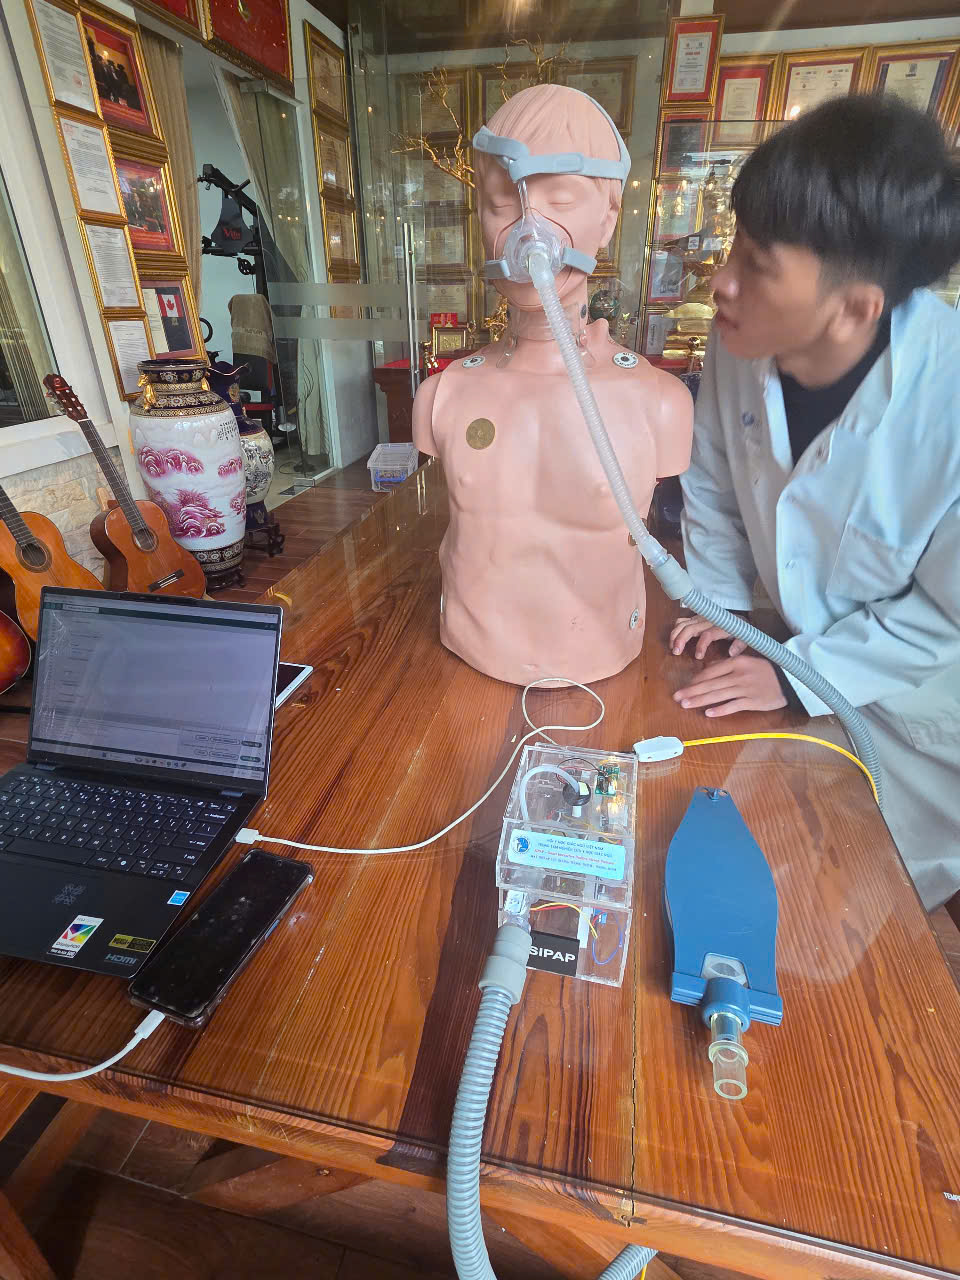
\includegraphics[width=0.7\textwidth]{image_2.png}
    \caption{Thử nghiệm thực nghiệm đo đạc thông số và điều khiển tốc độ quạt thổi trên mô hình người giả kết nối với máy tính.}
    \label{fig:fig9}
\end{figure}

% --- Section VI ---
\section{\textcolor{navy}{VI. HIỆU QUẢ ĐẠT ĐƯỢC VÀ ĐỊNH HƯỚNG PHÁT TRIỂN}}

\subsection{Hiệu quả kỹ thuật và kinh tế:}
\begin{itemize}
    \item \textbf{Giá thành chế tạo cực kỳ thấp:} Tổng chi phí linh kiện chỉ khoảng 7.345.000 VND, rẻ hơn từ 3 đến 8 lần so với các máy CPAP thương mại nhập khẩu trên thị trường.
    \item Hệ thống tích hợp các cảm biến đo lường áp suất và lưu lượng khí thở thời gian thực, cung cấp dữ liệu hô hấp quan trọng cho bệnh nhân trong giấc ngủ.
    \item \textbf{Khả năng IoT hóa cao:} Nhờ kết nối BLE và sự chuẩn bị của module ESP32, dữ liệu hô hấp có thể dễ dàng đồng bộ lên đám mây y tế SleepCare, cho phép bác sĩ chẩn đoán và theo dõi từ xa.
    \item Thiết kế nhỏ gọn, vỏ mica cắt laser trong suốt giúp dễ dàng kiểm tra cơ khí trực quan, lắp đặt và sửa chữa nhanh chóng theo dạng module.
\end{itemize}

\subsection{Lộ trình định hướng phát triển (Đưa vào nghiên cứu lâm sàng của VSSM):}
\begin{itemize}
    \item \textbf{Giai đoạn 1: Clinical Trial \& Safety Certifications} - Tiến hành thử nghiệm lâm sàng mẫu thử nghiệm để đánh giá độ an toàn y tế và hiệu chuẩn dải áp lực tối ưu dưới sự giám sát của GS.TS.KH. Dương Quý Sỹ.
    \item \textbf{Giai đoạn 2: Cloud Integration \& Remote Monitoring} - Hoàn thiện firmware cho vi điều khiển phụ ESP32 để kết nối Wi-Fi, đẩy dữ liệu trực tiếp lên cloud server mà không cần thông qua điện thoại trung gian.
    \item \textbf{Giai đoạn 3: AI-based Adaptation} - Phát triển và nhúng thuật toán trí tuệ nhân tạo (AI/Machine Learning) trên ứng dụng di động hoặc máy chủ để tự động nhận dạng nhịp thở bất thường và đưa ra dự báo sớm cơn ngưng thở, từ đó điều chỉnh tự động áp suất quạt thổi (Auto-CPAP/APAP) thông minh hơn.
    \item \textbf{Giai đoạn 4: Sleep Ecosystem Integration} - Tích hợp thiết bị vào hệ sinh thái chăm sóc giấc ngủ thông minh toàn diện cùng các cảm biến môi trường (nhiệt độ, ánh sáng, tiếng ồn phòng ngủ).
\end{itemize}

\begin{figure}[h!]
    \centering
    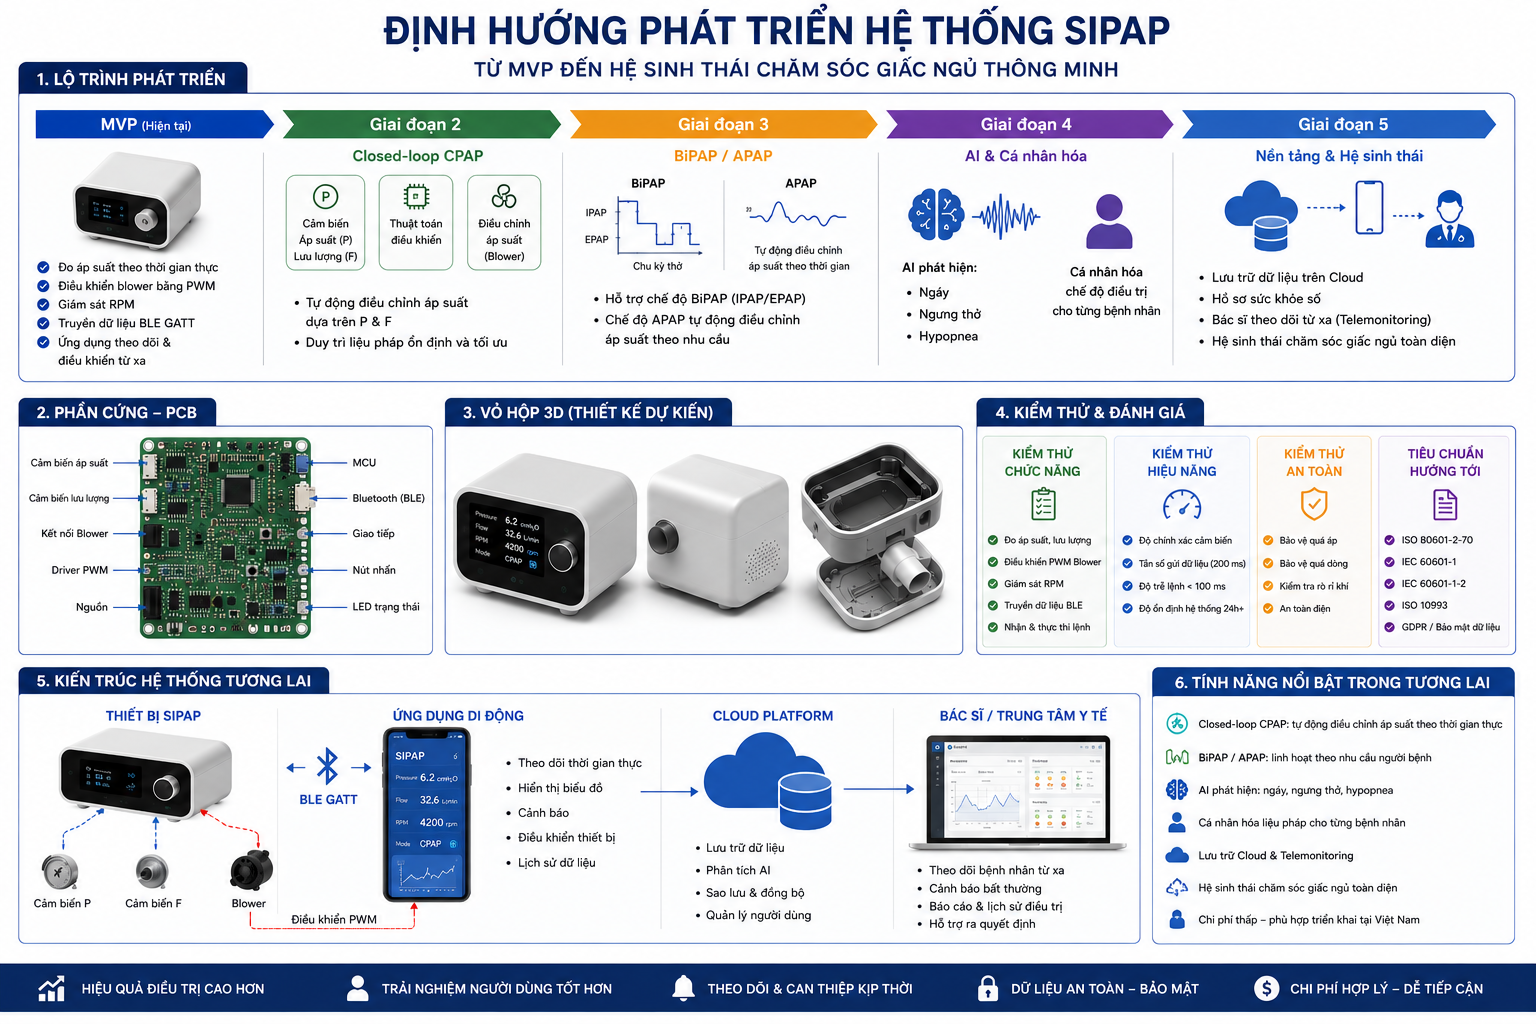
\includegraphics[width=0.8\textwidth]{image_5.png}
    \caption{Sơ đồ lộ trình phát triển hệ thống SIPAP từ phiên bản thử nghiệm (MVP) đến hệ sinh thái chăm sóc giấc ngủ thông minh (Mô hình mô phỏng thiết kế dự kiến).}
    \label{fig:fig10}
\end{figure}

% --- Section VII ---
\section{\textcolor{navy}{VII. YÊU CẦU BẢO HỘ}}

\begin{enumerate}
    \item Hệ thống hỗ trợ thở áp lực dương liên tục (CPAP) tương tác thông minh (SIPAP) dùng trong hỗ trợ điều trị hội chứng ngưng thở khi ngủ, hệ thống bao gồm:
    \begin{itemize}
        \item Một khối tạo áp lực dương gồm quạt thổi không chổi than 12VDC và bộ điều khiển tốc độ bằng xung PWM;
        \item Một khối cảm biến đo lường tích hợp gồm cảm biến áp suất analog kết nối qua cầu phân áp để giám sát áp suất mặt nạ thở, và cảm biến lưu lượng dòng khí giao tiếp chuẩn I2C;
        \item Một khối vi điều khiển trung tâm tích hợp module truyền thông Bluetooth Low Energy (BLE), được kết nối điện với khối tạo áp lực và khối cảm biến;
        \item \textbf{Đặc trưng ở chỗ:} Vi điều khiển trung tâm được lập trình để liên tục đọc tín hiệu áp suất mặt nạ thở từ cảm biến áp suất, tính toán lưu lượng từ cảm biến dòng khí, đồng thời đo tốc độ quay RPM của quạt thổi thông qua đếm số lượng xung phản hồi tốc độ quay nối vào chân ngắt ngoài của vi điều khiển, và định kỳ truyền chuỗi dữ liệu định dạng JSON chứa các thông số áp suất, RPM và giá trị PWM quạt thổi qua giao tiếp BLE GATT Profile dưới tên quảng bá 'SIPAP' để giám sát thời gian thực.
    \end{itemize}
    
    \item Hệ thống hỗ trợ thở theo điểm yêu cầu bảo hộ 1, \textbf{đặc trưng ở chỗ:} Thiết kế phần cứng tích hợp sẵn cổng kết nối chờ và thiết lập mã nguồn dự phòng để tích hợp cảm biến đo nồng độ bão hòa oxy máu $SpO_2$ quang học ở phiên bản nâng cấp.
    
    \item Hệ thống hỗ trợ thở theo điểm yêu cầu bảo hộ 1 hoặc 2, \textbf{đặc trưng ở chỗ:} Vi điều khiển trung tâm được cấu hình tính năng bảo vệ an toàn tự động ngắt quạt thổi (đặt PWM = 0) ngay lập tức khi phát hiện mất kết nối không dây BLE với ứng dụng di động.
    
    \item Hệ thống hỗ trợ thở theo điểm yêu cầu bảo hộ 1, \textbf{đặc trưng ở chỗ:} Vỏ máy thở và buồng chứa quạt tạo áp lực dương được chế tạo nguyên khối từ các tấm mica trong suốt cắt laser có độ dày từ 3-5mm để đảm bảo độ kín khí và khả năng quan sát trực quan các thành phần phần cứng bên trong.
    
    \item Hệ thống hỗ trợ thở theo điểm yêu cầu bảo hộ 1, \textbf{đặc trưng ở chỗ:} Hệ thống tích hợp thêm một bình làm ẩm khí thở (Humidifier) chứa nước cất y tế đặt tiếp nối sau khối tạo áp lực dương và trước mặt nạ thở, nhằm làm ẩm tự nhiên luồng khí lưu thông, ngăn ngừa hiện tượng khô rát niêm mạc hô hấp của người sử dụng.
    
    \item Hệ thống hỗ trợ thở theo điểm yêu cầu bảo hộ 1, \textbf{đặc trưng ở chỗ:} Bảo hộ tên gọi độc quyền sáng chế 'SIPAP' (Smart Interactive PAP - Thiết bị hỗ trợ thở áp lực dương tương tác thông minh) do GS.TS.KH. Dương Quý Sỹ đề xuất sáng tạo gắn liền với hệ sinh thái giải pháp kỹ thuật y tế nêu trên.
\end{enumerate}

\end{document}
